\documentclass[a4paper, landscape, 10pt]{article}

\usepackage{graphicx}
\usepackage{color}
\usepackage{tikz}
\usepackage{pgfplots}
\usepackage{pgf-umlsd}
\usepackage{ifthen}

\begin{document}
\title{VAE Ca Volume Prediction}
\begin{figure}
	\noindent\resizebox{\textwidth}{!}{
	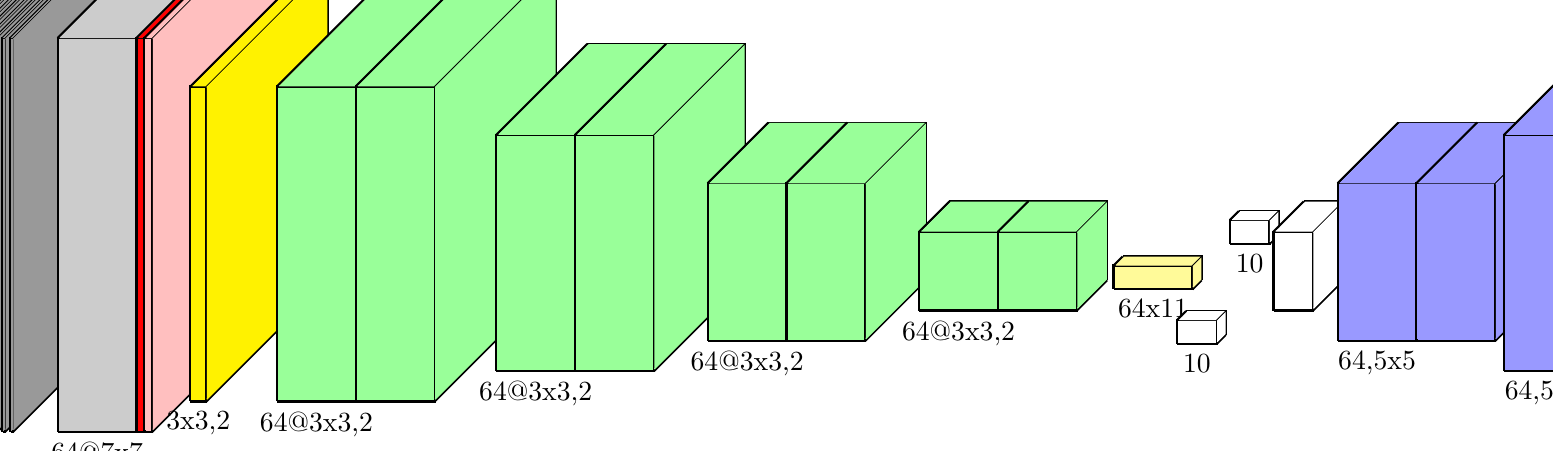
\begin{tikzpicture}
		\draw[use as bounding box, transparent] (-1.8,-1.8) rectangle (17.2, 3.2);

		% Define the macro.
		% 1st argument: Height and width of the layer rectangle slice.
		% 2nd argument: Depth of the layer slice
		% 3rd argument: X Offset --> use it to offset layers from previously drawn layers.
		% 4th argument: Options for filldraw.
		% 5th argument: Text to be placed below this layer.
		% 6th argument: Y Offset --> Use it when an output needs to be fed to multiple layers that are on the same X offset.

		\newcommand{\networkLayer}[6]{
			\def\a{#1} % Used to distinguish input resolution for current layer.
			\def\b{0.02}
			\def\c{#2} % Width of the cube to distinguish number of input channels for current layer.
			\def\t{#3} % X offset for current layer.
			\def\d{#4} % Y offset for current layer.

			% Draw the layer body.
			\draw[line width=0.3mm](\c+\t,0,\d) -- (\c+\t,\a,\d) -- (\t,\a,\d);                                                      % back plane
			\draw[line width=0.3mm](\t,0,\a+\d) -- (\c+\t,0,\a+\d) node[midway,below] {#6} -- (\c+\t,\a,\a+\d) -- (\t,\a,\a+\d) -- (\t,0,\a+\d); % front plane
			\draw[line width=0.3mm](\c+\t,0,\d) -- (\c+\t,0,\a+\d);
			\draw[line width=0.3mm](\c+\t,\a,\d) -- (\c+\t,\a,\a+\d);
			\draw[line width=0.3mm](\t,\a,\d) -- (\t,\a,\a+\d);

			% Recolor visible surfaces
			\filldraw[#5] (\t+\b,\b,\a+\d) -- (\c+\t-\b,\b,\a+\d) -- (\c+\t-\b,\a-\b,\a+\d) -- (\t+\b,\a-\b,\a+\d) -- (\t+\b,\b,\a+\d); % front plane
			\filldraw[#5] (\t+\b,\a,\a-\b+\d) -- (\c+\t-\b,\a,\a-\b+\d) -- (\c+\t-\b,\a,\b+\d) -- (\t+\b,\a,\b+\d);

			% Colored slice.
			\ifthenelse {\equal{#5} {}}
			{} % Do not draw colored slice if #4 is blank.
			{\filldraw[#5] (\c+\t,\b,\a-\b+\d) -- (\c+\t,\b,\b+\d) -- (\c+\t,\a-\b,\b+\d) -- (\c+\t,\a-\b,\a-\b+\d);} % Else, draw a colored slice.
		}

		% INPUT
% 		\node[] (input image) at (-3.75,0.5) {\includegraphics[height=30mm]{lenna.png}};
		\networkLayer{5.0}{0.03}{-1.1}{0.0}{color=gray!80}{$Volume_t$}
        \foreach \x in {1,...,10}{
          \networkLayer{5.0}{0.03}{-1.1+0.1*\x}{0.0}{color=gray!80}{}
        }

		% ENCODER
		\networkLayer{5.0}{1.0}{0.5}{0.0}{color=gray!40}{64@7x7}    % S1
		\networkLayer{5.0}{0.1}{1.5}{0.0}{color=red}{}        % S2
        \networkLayer{5.0}{0.1}{1.6}{0.0}{color=pink}{}        % S2
		\networkLayer{4.0}{0.2}{1.8}{0.0}{color=yellow}{3x3,2}    % S1

        \networkLayer{4.0}{1.0}{2.9}{0.0}{color=green!40}{64@3x3,2}
        \networkLayer{4.0}{1.0}{3.9}{0.0}{color=green!40}{}
        \networkLayer{3.0}{1.0}{5.3}{0.0}{color=green!40}{64@3x3,2}
        \networkLayer{3.0}{1.0}{6.3}{0.0}{color=green!40}{}
        \networkLayer{2.0}{1.0}{7.6}{0.0}{color=green!40}{64@3x3,2}
        \networkLayer{2.0}{1.0}{8.6}{0.0}{color=green!40}{}
        \networkLayer{1.0}{1.0}{9.9}{0.0}{color=green!40}{64@3x3,2}
        \networkLayer{1.0}{1.0}{10.9}{0.0}{color=green!40}{}

        \networkLayer{0.3}{1.0}{12.1}{0.0}{color=yellow!40}{64x11}

        \networkLayer{0.3}{0.5}{13.6}{1.8}{color=white}{10}
        \networkLayer{0.3}{0.5}{13.0}{-1.5}{color=white}{10}

        \networkLayer{1.0}{0.5}{14.4}{0.0}{color=white}{}

        \networkLayer{2.0}{1.0}{15.6}{0.0}{color=blue!40}{64,5x5}
        \networkLayer{2.0}{1.0}{16.6}{0.0}{color=blue!40}{}
        \networkLayer{3.0}{1.0}{18.1}{0.0}{color=blue!40}{64,5x5}
        \networkLayer{3.0}{1.0}{19.1}{0.0}{color=blue!40}{}
        \networkLayer{4.0}{1.0}{20.6}{0.0}{color=blue!40}{64,5x5}
        \networkLayer{4.0}{1.0}{21.6}{0.0}{color=blue!40}{}
        \networkLayer{5.0}{1.0}{23.1}{0.0}{color=blue!40}{64,5x5}
        \networkLayer{5.0}{1.0}{24.1}{0.0}{color=blue!40}{}

		% OUTPUT
		\networkLayer{5.0}{0.03}{25.7}{0.0}{color=gray!80}{$Volume_{t}$}
        \foreach \x in {1,...,10}{
          \networkLayer{5.0}{0.03}{25.7+0.1*\x}{0.0}{color=gray!80}{}
        }
% 		\node[] (output image) at (18,0.5) {\includegraphics[height=30mm]{vermeer.jpg}};


	\end{tikzpicture}
	}
	\caption{Convolution (Light gray), Batch Norm (Red), Relu (Pink), Max Pool (Yellow), Resnet block (Green), Average Pool (light yellow), Dense (white), Super Resolution (Blue)}
	\label{fig:cnn}
\end{figure}

\end{document}
